\documentclass[a4paper,10pt]{article}
\usepackage[T1]{fontenc}
\usepackage[utf8]{inputenc}
\usepackage[english]{babel}
\usepackage{lmodern}
\usepackage[top=1.6cm,bottom=1.8cm,left=1.9cm,right=1.9cm]{geometry}
\usepackage{titlesec,enumitem,xcolor,graphicx,lastpage,fancyhdr}
\usepackage{fontawesome5}
\usepackage[hidelinks]{hyperref}

\hypersetup{colorlinks=true,urlcolor=blue!70!black,linkcolor=blue!70!black}
\pagestyle{fancy}\fancyhf{}\renewcommand{\headrulewidth}{0pt}
\fancyfoot[C]{\small\color{gray}Page \thepage\ of \pageref{LastPage}}
\setlength{\parindent}{0pt}

\titleformat{\section}{\large\bfseries\color{blue!70!black}}{}{0em}{}[\vspace{-0.7em}\rule{\textwidth}{0.5pt}]
\titlespacing{\section}{0pt}{9pt}{5pt}
\setlist[itemize]{leftmargin=1.1em,itemsep=2pt,topsep=2pt,parsep=0pt}
\newcommand{\role}[4]{\vspace{3pt}\noindent\hspace{0.6em}\parbox[t]{0.38\textwidth}{\raggedright\textbf{#1}}\hfill\parbox[t]{0.58\textwidth}{\raggedleft\textit{#2}}\\{\textit{#3}\hfill\textit{#4}}\vspace{1pt}}

\begin{document}
\noindent
\begin{minipage}[t]{0.78\textwidth}
\vspace{0pt}
{\huge\bfseries Prabhavit Gupta}\\[8pt]
{\small \faPhone\ +39-351-610-7807 \quad \faEnvelope\ \href{mailto:prabhavitg@gmail.com}{prabhavitg@gmail.com} \quad \faLinkedin\ \href{https://www.linkedin.com/in/prabhavit/}{Linkedin} \quad \faMapMarker*\ Venice, Italy}
\end{minipage}\hfill
\begin{minipage}[t]{0.18\textwidth}
\vspace{0pt}\raggedleft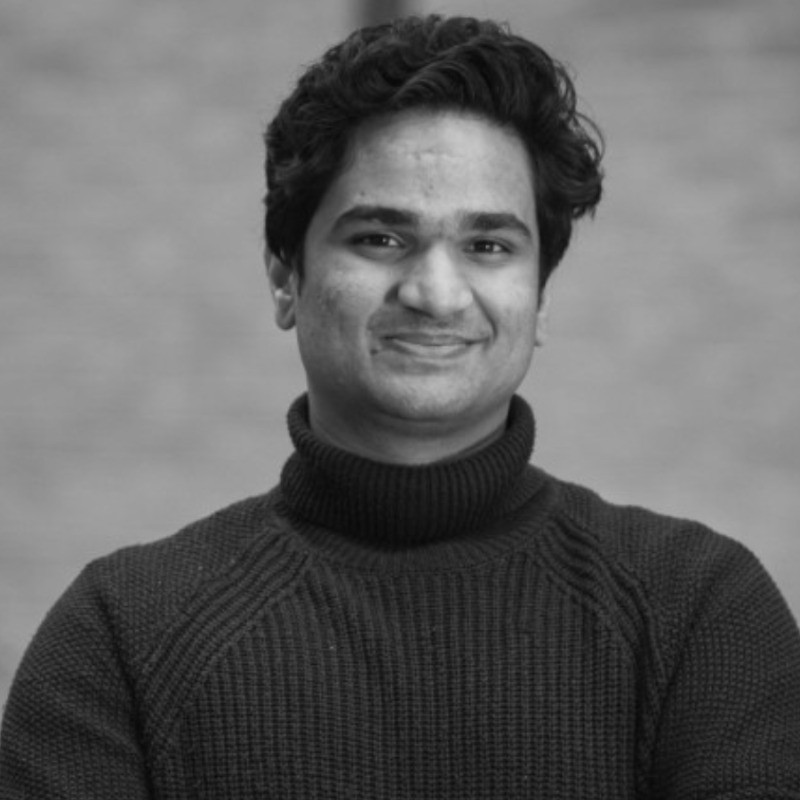
\includegraphics[width=2.3cm,height=2.3cm,keepaspectratio]{photo.jpg}
\end{minipage}

\section{Career Summary}
\begin{itemize}
\item AI Engineer with hands-on experience building robust, scalable LLM-driven applications and agentic workflows across European tech projects.
\item Skilled in developing AI agents (RAG, Microsoft Agent concepts), prompt engineering, and orchestrating complex end-to-end data pipelines.
\item Strong product engineering mindset with full-stack capabilities (Frontend/Backend), transforming business requirements into production-ready AI solutions.
\end{itemize}

\section{Technical Skills}
\begin{itemize}
\item \textbf{AI/ML} -- AI Agents, LangChain concepts, RAG, API integration, Eden AI, OpenAI integration
\item \textbf{Automation} -- n8n, Playwright, ML workflows
\item \textbf{Development} -- Claude Code, Laravel, Typescript, Full-stack Product Engineering
\item \textbf{Project/Design} -- AI observability, Figma, Jira, GitHub, Postman
\end{itemize}

\section{Visa \& Language}
\begin{itemize}
\item \textbf{Language} -- Hindi (Native), English (Professional), Italian (Beginner)
\item \textbf{Work Authorization} -- European Long Term Residence Permit - No Sponsorship required.
\end{itemize}

\section{Professional Experience}
\role{\href{https://flowspace.co}{FlowSpace.co}}{Lead Developer (Full time, Freelance)}{London, UK}{Mar 2024 -- Ongoing}
\begin{itemize}
\item \textbf{Product Responsibilities:}
\begin{itemize}[label=--]
\item Scaled platform from 2000 to 4500+ users through iterative product development and end-to-end pipelines.
\item Overseeing the migration of app from Bubble.io to Next.JS and Laravel.
\item Collaborated with cross-functional team of developers for product logic and business logic documentation.
\item Streamlined customer support with AI agents.
\end{itemize}
\item \textit{Tools: Playwright, Jira, Google Analytics, Microsoft Clarity}
\item \textbf{Technical Responsibilities:}
\begin{itemize}[label=--]
\item Architected an AI tool for processing and scraping of data, increasing listings and optimising for reliability.
\item Consolidated leads in CRM and automated lead capture by developing integrations between CRM systems.
\item GTM automations for sales funnel, lead enrichment and outbound.
\item \textit{Tools: Claude Code, n8n, Postman, Jira, Github, Laravel, Typescript}
\end{itemize}
\end{itemize}

\role{Urlink}{Project Manager and AI Assisted Developer (Freelance)}{Barcelona, Spain}{April 2025 -- July 2025}
\begin{itemize}
\item Architected agentic solutions for building platform logics and robust UIs.
\item Implemented automations and workflows tailored to specific client requirements and UX constraints.
\item \textit{Tools: Github, Netlify, Supabase, bolt.new}
\end{itemize}

\role{UltraStrategy.com}{Automation Developer (Collaborator)}{France}{Dec 2024 -- May 2025}
\begin{itemize}
\item Developed a scalable CV parsing AI tool using n8n and Eden AI for end-to-end data processing.
\item \textit{Tools: n8n, Eden AI, Bubble.io}
\end{itemize}

\role{Get2Germany.com}{Lead Developer and Automation Specialist (Part time)}{Berlin, Germany}{Jan 2024 -- May 2024}
\begin{itemize}
\item Integration of Google APIs for effective tracking of the platform and database optimization.
\item Developed AI-based automation tools for parsing and finding courses, internships, and jobs.
\item \textit{Tools: Bubble.io, Figma, Trello, n8n}
\end{itemize}

\role{Clubee.com}{Low Code Developer and Quality Assurance (Full time, Freelance)}{Foetz, Luxembourg}{Sep 2023 -- Aug 2024}
\begin{itemize}
\item Integration of Clubee API for all frontend functionality.
\item Performed unit testing and quality assurance of new features to validate system behaviour.
\item \textit{Tools: Bubble.io, Figma, GitHub, Postman}
\end{itemize}

\section{Education}
\role{Ca' Foscari University of Venice}{Bachelor's in Philosophy, International Studies \& Economics with Minor in Entrepreneurship}{Venice, Italy}{Oct 2020 -- Jun 2024}

\section{Certifications}
\begin{itemize}
\item Microsoft Copilot Studio Agent Academy
\item Microsoft - Introduction to building AI agents
\item Microsoft Power Automate
\item Tray.AI Build Practitioner -- September 2024
\item Tray.AI Build Foundations
\end{itemize}

\end{document}
